% Created 2019-05-13 Mon 19:29
% Intended LaTeX compiler: pdflatex
\documentclass[12pt, a4paper]{report}
\usepackage[utf8]{inputenc}
\usepackage[T1]{fontenc}
\usepackage[czech, ]{babel}
\usepackage{graphicx}
\usepackage{grffile}
\usepackage{longtable}
\usepackage{float}
\usepackage{wrapfig}
\usepackage{rotating}
\usepackage[normalem]{ulem}
\usepackage{amsmath}
\usepackage{textcomp}
\usepackage{amssymb}
\usepackage{capt-of}
\usepackage[hidelinks]{hyperref}
\usepackage{csquotes}
\usepackage{tabularx}
\MakeOuterQuote{"}
\usepackage{setspace}
\onehalfspacing
\usepackage{titlesec}
\titleformat{\chapter}[display]{\normalfont\bfseries}{}{0pt}{\Huge}
\usepackage[backend=bibtex,citestyle=authoryear]{biblatex}
\addbibresource{~/OneDrive/Orgmode/Papers/references.bib}


\DeclareUnicodeCharacter{00A0}{~}
% \addbibresource{./references/references.bib} % pro pouziti lokalni slozky se zdroji
\author{Matěj Haša, Vít Chrubasík, Marek Štěpán}
\date{Květen 2019}
\title{Projekt: Státní maturita s Khan Academy\\\medskip
\large 
\includegraphics[width=\linewidth]{./images/skola_logo.png} Seminární práce}
\hypersetup{
 pdfauthor={Matěj Haša, Vít Chrubasík, Marek Štěpán},
 pdftitle={Projekt: Státní maturita s Khan Academy},
 pdfkeywords={},
 pdfsubject={},
 pdfcreator={Emacs 26.1 (Org mode 9.2.3)}, 
 pdflang={Czech}}
\begin{document}

\maketitle
\tableofcontents
\thispagestyle{empty}
\listoftables
\thispagestyle{empty}
\listoffigures
\thispagestyle{empty}



\chapter{Úvod}
\label{sec:org14094a2}
V této seminární práci se budeme snažit co nejlépe aplikovat nabyté vědomosti,
získané z hodin kurzu Projektové řízení A, které se týkají úvodní fáze projektu.
V této fázi se, především, projekt plánuje, analyzuje a ověřuje se, jestli je
proveditelný v kontextu našich možných zdrojů, efektivní \emph{et cetera}.

\section{Co je Khan Academy?}
\label{sec:org22c7301}
\phantomsection
\label{orge0f9e9b}
\begin{quote}
"You can learn anything."

-- Salman Khan, zakladatel Khan Academy
\end{quote}

Khan Academy je webová vzdělávací platforma. Citát samotný je mottem Khana i celé
organizace a výstižně shrnuje poslání Khan Academy, kterým je vysoce kvalitní
vzdělání pro všechny, všude a zdarma.

Ve svém TED Talku "\citetitle{khan_ted_historie}" Salman Khan mluví o začátcích Khan
Academy. Říká, že vzdělávací platformu nikdy založit neplánoval. Před Khan
Academy pracoval jako analytik v hedgeovém fondu a jednoho dne ho oslovili jeho
příbuzní \footnote{Pozn. k překladu: bratranci nebo sestřenice, pohlaví ani počet
z anglického projevu nevyplývá} s tím, že by potřeboval doučit témata ze
středoškolské matematiky. Sal Khan chtěl rodině pomoci, ale příbuzní žili
daleko, a proto k pravidelným schůzkám nemohlo docházet. Sala tenkrát napadla
brilantní myšlenka a to, že přednahraje lekce z matematiky a dá je jako videa na
platformu YouTube. "They told me that they preferred me on YouTube than in
person\ldots{}" vtipně poznamenal Khan, ale subtext této věty potom vysvětlil tím, že
lekce z videí jsou zastavit či přehrát opakovaně. A videu nevadí, když něčemu
nerozumíte, klidně se vám přehraje, kolikrát jen budete chtít.

\section{Matematika na Khan Academy}
\label{sec:org6ff349a}
V dalším TED Talku s názvem \citetitle{khan_ted_mastery} Khan osvětluje ideu, která má
přispět k pokroku ve vyučování, především ve vyučování matematiky. Khan využívá
pro současné vzdělávání následující analogie, kterou se pokusíme co nejvěrněji
parafrázovat.

Představte si, že chodíte do školy a v jedné lekci se učíte jízdě na kole.
Nejprve před vás postaví kolo a ukáží vám, jak se na něm jezdí a zbytek nechají
na vás s tím, že za týden bude test z jízdy na 200 metrů. Za týden je, skutečně,
test, ve kterém předvádíte, jak jste se naučili jezdit. Moc vám to nejde,
párkrát spadnete, a nakonec ujedete 100 metrů. Tak jste splnili test na 50 \%,
a dostanete za C. Potom přijdete na další lekci, kde před vás postaví
jednokolku\ldots{} Jestli si říkáta, jak se asi máte naučite na jednokolce za týden,
když jste se za týden pořádně nenaučili držet rovnováhu ani na kole, tak s vámi
Sal Khan souhlasí a ptá se "tak proč tímto způsobem vyučujeme matematiku?"
Jestliže chcete v matematice pokročit, musíte nejdříve umět dokonale látku
předhozí, jinak to nejde. \parencite{khan_ted_mastery}

Khan potom představuje systém, ve kterém se matematika vyučuje tak, že skrze
intenzivní testy na webu jsou prověřeny znalosti matematiky, které jsou předtím
vyučovány formou video-lekcí a k další látce se postupuje po dokonalém ovládnutí
předhozího konceptu. Nenastávají tak mezery ve vzdělání. Ohlasy na tento styl
výuky jsou velmi pozitivní.

Organizace samotná je vedena jako nezisková, je, však,
dotována mnoha sponzory, mezi kterými je například i Bill \& Melinda Gates
Foundation \parencite{khan_academy_supp}.


\section{Projekt}
\label{sec:org6c4e333}

Náš fiktivní projekt má za cíl implementovat výukové materiály pro českou
státní maturitu do již existující online vzdělávací platformy Khan Academy.
V aktuálním řešení (Květen 2019) jsou dostupné kurzy z většiny vědních oborů
jako např.: matematiky, biologie, chemie, fyziky, historie \emph{et cetera}. Khan
Academy je dostupná i v českém jazyce. S týmem bychom chtěli vytvořit projekt,
jehož obsahem bude rozšíření výukových materiálů na verzi s českou jazykovou
mutací a to o výukové materiály pro českou státní maturitu z matematiky.

\chapter{Identifikační listina}
\label{sec:orge003a70}
V této kapitole můžete zhlédnout identifikační listinu, kterou jsme vytvořili za
účelem uceleného přehledu o našem projektu. V listině jsme uvedli všechny
klíčové parametry jako jasně definovaný cíl a účel projektu, rozdělení
zodpovědností či milníky průběhu projektu, které nám budou jasně indikovat, že
je čas měřit a ověřit část dosavadních výsledků projektu.

\begin{table}[htbp]
\caption{\textbf{Identifikační listina projektu}}
\centering
\footnotesize
\begin{tabularx}{\textwidth}{lX}
\textbf{Název projektu:} & Státní maturita s Khan Academy\\
\textbf{Obsah:} & Přidání přípravných kurzů ke státní maturitní zkoušce z matematiky do platformy Khan Academy\\
\textbf{Účel:} & Poskytnutí možnosti kvalitní přípravy ke státní maturitní zkoušce z matematiky\\
\textbf{Cíle projektu:} & 1. Zavést plnohodnotný kurz do již existující platformy, jehož výstupem bude člově schopný úspěšně vykonat státní maturitní zkoušku za matematiky\\
 & 2. Zvýšit úspěšnost u maturitní zkoušky za matematiky\\
 & 3. Motivovat účastníky kurzu k dalšímu studio, které zahrnuje matematiku\\
\textbf{Termín zahájení:} & Leden 2020\\
\textbf{Termín ukončení:} & Září 2021\\
\textbf{Vedoucí projektu:} & Vít Chrubasík\\
\textbf{Členové projektového týmu:} & Matěj Haša, Marek Štěpán\\
\textbf{Garant:} & Vít Chrubasík\\
\textbf{Milníky:} & viz \cite{ms_project_soubor}\\
\end{tabularx}
\end{table}


\chapter{Logický rámec}
\label{sec:org4678299}

\begin{table}[htbp]
\caption{\textbf{Logický rámec}}
\centering
\footnotesize
\begin{tabularx}{\textwidth}{|X|X|X|X|}
\hline
Sloupec intervencí & Objektivně měřitelný ukazatel & Zdroje informací k ověření & Rizika / předpoklady (vnější)\\
\hline
Zvýšit úspěšnost u státní maturity z matematiky & Absolventi kurzu & Dotazníky, výsledky absolventů & \\
\hline
Poskytnutí možnosti dobré přípravy ke zkoušce & Absolventi kurzu & Statistické údaje & Správně sestavený kurz, který se osvědčil v dobré přípravě studentů\\
\hline
Sekce Maturita na na české Khan Academy & Beta-testování, testovací a  kontrolní skupina & reporty z testování & Validní testovací scénáře, úspěšná fáze testování, statisticky významné zlepšení testovací skupiny\\
\hline
Návrh, implementace, testování, nasazení, údržba & Lidská práce, know-how, hardware, technologie, energie & Vedoucí pracovníci, road map, účetní výkazy & Správná analýza, kvalitní vývojová platforma, dobře fungující tým\\
\hline
 &  &  & Svolení k realizaci projektu ze strany Khan Academy\\
\hline
\end{tabularx}
\end{table}

\chapter{SWOT analýza}
\label{sec:org7b81b8a}
Před samotnou realizací projektu jsme si sepsali naše silné a slabé stránky,
příležitosti i hrozby. Vytvořili jsme analýzu SWOT. Jsme si vědomi faktu, že je
v našich silách ovlivnit jak naše slabé tak silné stránky. Hrozeb je třeba se
vyhnout.

V případě našeho projektu jednoznačné pozitivum vidíme v integraci našeho řešení
do již zaběhlé a fungující platformy. Nejen, že tato služba má již své klienty,
ale také IT řešení již má fungující platformu. Budeme nabízet veřejně prospěšnou
činnost, což se v dněšní době sociálně marketingové koncepce nosí. Lidé zkrátka
slyší na produkty, jejichž zájem je sladěn s dlouho\-dobými sociálními a
etickými zájmy celé společnosti. Služba je na českém trhu originální. Existují
youtubeři a domácí lektoři, kteří se snaží připravovat studenty na úspěšné
zvládnutí maturitní zkoušky z matematiky, ale nikdo nenabízí komplexní řešení
krok po kroku, jako my.

Slabé stránky vidíme v našem týmu, který je poměrně malý a nezkušený. Ani jeden
z nás nemá zkušenosti s podobným projektem. Ruku v ruce s tímto tvrzením jde
i malý rozpočet, který především v pozdějších fázích projektu může být problém
a výsledný produkt se může začít ochuzovat o potřebné fáze jako např.: důsledné
testování. Budeme se snažit náš tým přetransformovat z nezkušených nováčků na
tomto trhu na inovativní skupinu, která může přinést nové nápady či řešení
v odvětví online vzdělávání.

Když přijde na příležitosti našeho projektu, myslíme si, že vzhledem k jeho
dobrým účelům, o kterých jsme hovořili v silných stránkách, může chtít přispět k
vývoji řada dobrovolníků. Také budeme aktivní na poli žádostí o dotace.

Po důkladné analýze jsme vyčlenili čtyři nejzávažnější hrozby. Mohou přijít
změny ze strany Ministerstva školství a to, jak v aktuálních osnovách maturity
tak v úplném zrušení státní maturitní zkoušky. Této hrozbě nijak předejít nejde,
pravděpodobnost zrušení státní zkoušky je naštěstí malá. Změnit osnovy se mohou
a na tuto hrozbu jsme připraveni -- budeme iterativně kontrolovat oficiální
požadavky na studenty a na jejich základě pružně reagovat na potenciální změny.
Samozřejmě, i nám se nevyhne riziko možných konkurenčních bojů, ale spolu
s kolegy se této skutečnosti příliš neobáváme. Khan Academy si drží značnou část
trhu (protože je naprosto zdarma) a nic nenaznačuje změnám v blízké budoucnosti.
Může se stát, že top management Khan Academy s námi odmítne spolupracovat --
budeme se snažit projekt uvést v co možná nejlepším světle, abychom tuto hrozbu
snížili na minimální hodnotu.

Pro ucelený kvatnifikovaný přehled můžete nahlédnout do tabulky \ref{tab:swot}.

\begin{table}[htbp]
\caption{\label{tab:org5202e4b}
\textbf{SWOT analýza}}
\centering
\footnotesize
\begin{tabularx}{\textwidth}{|X|r|r|r|}
\hline
Položka & Váha & Hodnocení & Hodnota\\
\hline
\textbf{Silné stránky} &  &  & \\
Materiálová nenáročnost & 10 & 2 & 0.2\\
Veřejně prospěšná činnost & 20 & 3 & 0.6\\
Originalita & 30 & 5 & 1.5\\
Implementace do zaběhnutého systému & 40 & 5 & 2.\\
\hline
\textbf{Silné stránky celkem} & 100 &  & 4.3\\
\hline
\textbf{Slabé stránky} &  &  & \\
Malý tým & 12 & 4 & -0.48\\
Nově sestavený tým & 20 & 1 & -0.2\\
Nizký rozpočet & 33 & 2 & -0.66\\
Málo praktických zkušeností & 35 & 3 & -1.05\\
\hline
\textbf{Slabé stránky celkem} & 100 &  & -2.39\\
\hline
\textbf{Příležitosti} &  &  & \\
Dotace & 25 & 2 & 0.5\\
Dobrovolníci & 47 & 4 & 1.88\\
Zvýšení poptávky & 12 & 1 & 0.12\\
Nefinanční příspěvky & 16 & 3 & 0.48\\
\hline
\textbf{Příležitosti celkem} & 100 &  & 2.98\\
\hline
\textbf{Hrozby} &  &  & \\
Změní se osnovy maturity & 35 & 3 & -1.05\\
Konkurence & 6 & 1 & -0.06\\
Odmítnutí návrhu implementace & 40 & 3 & -1.2\\
Zrušení státní maturity & 19 & 1 & -0.19\\
\hline
\textbf{Hrozby celkem} & 100 &  & -2.5\\
\hline
\textbf{Interní faktory} &  &  & 1.91\\
\textbf{Externí faktory} &  &  & 0.48\\
\hline
\textbf{Závěr} &  &  & \textbf{2.39}\\
\hline
\end{tabularx}
\end{table}

\chapter{Myšlenková mapa}
\label{sec:org4821ac4}

\begin{figure}[htbp]
\centering
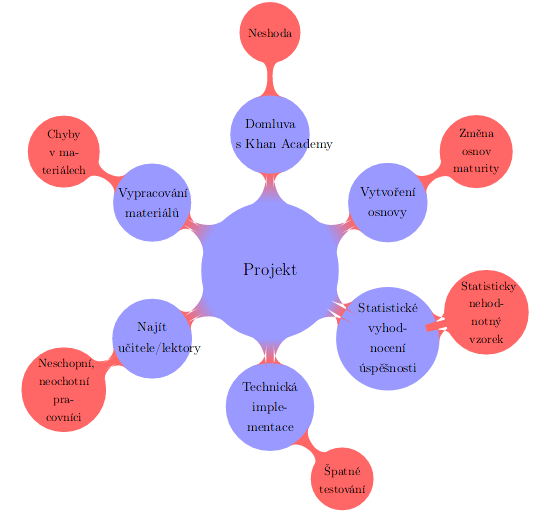
\includegraphics[width=.9\linewidth]{./images/myslenkova_mapa.png}
\caption[\textbf{Myšlenková mapa}]{\label{fig:org90a0a97}
V Myšlenkové mapě jsou zachyceny úkoly spojené s projektem společně s potenciálními riziky.}
\end{figure}


\chapter{Organizační plán projektu}
\label{sec:org0e23595}
Doplňkové materiály k organizačnímu plánu jsou dostupné v souboru \cite{ms_project_soubor}

\section{Work breakdown structure}
\label{sec:orgf836ddf}
Provedení projektu bylo rozděleno na 6 etap. Po sestavení a zaškolení týmu se
začne paralelně pracovat na vytváření osnovy a softwarové integraci do
existující platformy. Jakmile budou tyto etapy dokončeny, začne testovací fáze
s testovací skupinou, která bude následována vyhodnocením (tabulka \ref{tab:wbs1}
a \ref{tab:wbs2}).

\begin{table}[htbp]
\caption{\label{tab:org8959181}
\textbf{Work breakdown structure 1}}
\centering
\scriptsize
\begin{tabularx}{\textwidth}{|X|X|}
\hline
Etapa & Činnost\\
\hline
\textbf{Sestavení týmu} & Vytvoření inzerátů na pozice, které potřebujeme obsadit\\
\hline
 & Vedení pohovorů s kandidaty a vyhodnocení\\
\hline
 & Podepisování smluv, vyjednávání o podmínkách\\
\hline
 & Organizování teambuildingových aktivit pro stmelení týmu\\
\hline
 & Zaškolení, poučení o bezpečnosti atp.\\
\hline
 & Sestavení jednotlivých týmů a vytvoření organizační struktury\\
\hline
\textbf{Vytvoření osnovy} & Analýza požadavků\\
\hline
 & Vytvoření kostry témat a oblastní nutných pro zvládnutí maturitní zkoušky\\
\hline
 & Revize již sepsaných studijních plánů s týmem\\
\hline
 & Kontrola naší osnovy a porovnání s okruhy k maturitě\\
\hline
\textbf{Vypracování studijních materiálů} & Rozvržení jednotlivých osnov mezi týmy odborníků\\
\hline
 & Team leadeři jednotlivých týmů naplánují úkoly pro svůj tým\\
\hline
 & Zasazení naplánovaných úkolů do časového rámce a vytvoření submilníků\\
\hline
 & Tvoření a plnění jednotlivých úkolů, vytváření samotných studijních materiálů\\
\hline
 & Kontrola lingvistou, korektura překlepů\\
\hline
 & Najmutí skupiny studentů, kteří jsou ochotni podílet se na testování vypracovaných materiálů, dohodnutí podmínek\\
\hline
 & Testování materiálů od úzké skupiny studentů, sbíraní statistik a šetření dotazníky, hodnotí se srozumitelnost, přidaná hodnota kurzu celkově, odalují se nedostatky\\
\hline
 & Napravení všech nedostatků zjištěných při testování studentů\\
\hline
\end{tabularx}
\end{table}

\begin{table}[htbp]
\caption{\label{tab:org39c09d5}
\textbf{Work breakdown structure 2}}
\centering
\scriptsize
\begin{tabularx}{\textwidth}{|X|X|}
\hline
\textbf{Integrace do platformy Khan Academy} & Analýza použitých technologií v portále Khan Academy, tvoření struktury databáze\\
 & Sestavení UML diagramů, analýza budoucího rozšíření Khan Academy, tvoření struktury databáze\\
 & Vytváření tzv. Proof of Concept (PoC), kterým se ověří správnost analýzy zvoleného přístupu integrace do již existující platformy\\
 & Implementování technického řešení, kódování frontend a napojení na backend\\
 & Psaní UNIT testů, testování metod\\
 & Deployment do prostředí, spojení s již existující platformou\\
 & Doladění chyb a nepředvídaných problémů, které byly odhaleny již ve fázi vývoje a nasazení systému\\
\hline
\textbf{Testovací fáze} & Analýza use cases a vytvoření testovacích scénářů, určení priorit\\
 & Napsání akceptačních testů, performance testů\\
 & Vyhodnocování testů, ladění softwaru za neustálé komunikace s týmem vývojářů\\
 & Opětovný nábor skupiny studentů za účelem otestování aplikace, dohotnutí podmínek testování\\
 & Testování aplikace studenty, hledisko orientace v aplikaci, přehlednosti, black box testing\\
 & Vyhodnocení testovací fáze, určení kritických míst, analýza možné nápravy\\
\hline
\textbf{Vyhodnocení projektu} & Sběr dat z výsledků maturitních zkoušek od absolventů našeho kurzu\\
 & Vyhodnocení dat statisticky, vytvoření přehledných tabulek a grafů s daty\\
 & Porovnání s předhozím šetřením, s předešlými maturitami\\
 & Schůzka s investory a majiteli Khan Academy, diskuze o zpětné vazbě a rozšíření\\
 & Vyhodnocení zpětné vazby od všech aktérů na tomto projektu, poučení se do dalších projektů, analýza chyb\\
 & Sestavení reportu pro marketingové oddělení Khan Academy, začatek kampaně pro nadcházející ročník maturity\\
\hline
\end{tabularx}
\end{table}

\section{Kritická cesta}
\label{sec:orga55e7c7}
Projekt obsahuje celkem 36 činností, z toho 21 jich bylo identifi\-kováno jako
kritických

\begin{equation}
\label{eq:orgb4012fc}
 \frac{21}{36} \approx 58,33 \%
\end{equation}

Z vypočtu (\ref{eq:CI}) nám vyplývá index kritičnosti velmi přes 30 \%. Některé
činnosti budou vyžadovat odkritičnění v podobě využití časových rezerv
a realokaci zdrojů.

\section{Zdroje}
\label{sec:orgf09e652}
V projektu budou figurovat pouze lidské zdroje a náklady na ně budou spočteny
v podobě man-dayů, kdy jeden man-day reprezentuje pracovní směnu jednoho
člověka.


\section{Stakeholdeři}
\label{sec:orgd9ad19a}
\begin{itemize}
\item \textbf{Vedoucí projektu} -- Vít Chrubasík, má funkci jak top managera, tak
sponzora, zodpovídá se přímo Khan Academy a udává kurz projektu.
\item \textbf{Management} -- Jediná další úroveň managementu, Matěj Haša se Štěpánem
Markem, dohlíží na jednotlivé týmy.
\item \textbf{Týmoví pracovníci} -- Učitelé, lektoři, IT specialisté. Jsou důležitými
aktéry při realizaci projektu, hlavní část lidských zdrojů.
\item \textbf{Studenti a externisté} -- Testovací a kontrolní subjekty, studenti,
lingvisté, korektura. Ovlivňují testovací etapu.
\item \textbf{Zákazníci} -- Khan Academy a potenciální účastníci kurzu, buodu hlavním
aktérem při hodnocení projektu, primárně tito mají mají z projektu
benefitovat.
\end{itemize}


\chapter{Budoucí vývoj}
\label{sec:org09c777c}
Možnost budoucího vývoje vidíme v rozšíření přípravy i pro jiné předměty české
státní maturitní zkoušky. Jako iniciátoři projektu máme všichni matematiku rádi
a zároveň má tento předmět jedny z nejhorších úspěšnostních výsledků -- z tohoto
důvodu jsme se rozhodli připravovat studenty právě pro matematiku. Do budoucna
se však nebráníme rozšířit řešení i o Český jazyk, Anglický jazyk a další, třeba
i odborné předměty.

Je samozřejmostí, že pro další rozšíření aplikace mimo obor matematiky bychom
museli využít více externích pracovních sil z důvodu naší nedostatečné znalosti.
Zda-li navážeme dalším projektem, či dokonce projekty bude záležet na úspěšnosti
provedení tohoto, vyjednání podmínek s Khan Academy a oblíbenosti budoucí služby
obecně.

V daleké budoucnosti vidíme možnost i ve vzdělávání a přípravě na certifikáty a
kurzy obecně. Existují kurzy angličtiny jako např. FCE, certifikáty pro přehled
o testování software ISTQB a jistě plno dalších z mnoha oborů. Většinou již
existují přípravné knihy jak fyzické tak elektronické, ale těžko se vyrovnají
vedenému digitálnímu průvodci, který studenta vede krok po kroku a vše důkladně
vysvětluje. Student má také snadno dostupné diskusní fórum, kde případné
problému může okamžite konzultovat se svými kolegy. Z tohoto důvodu si myslíme,
že výše zmíněné navázání by za jistých okolnosti určitě mělo smysl.

\chapter{Závěr}
\label{sec:org259fe00}
Ačkoliv jsme se celou dobu pohybovali spíše v teoretické rovině, získali jsme
povědomí o tom, co všechno řízení projektu může obnášet. Jako semi-praktické
cvičení nám potom prospěl metaprojekt zpracování této seminární práce.

Mít pasivní znalost projektového řízení v dnešním světě shledáváme prerekvizitou
pro současný trh práce, kde se projekty objevují stále častěji. Obzvláště pak na
poli informačních technologií.

I kdybychom v budoucnu profesionálně projekty neřídili a byli bychom pouze
"řízeni," naše povědomí o projektovém řízení z nás udělá kompatibilního týmového
pracovníka na kterékoliv pozici.



\printbibliography
\end{document}